\chapter{Введение}  

Ряд исследований последнего времени демонстрируют уверенную корреляцию между ростом цен на нефть и объемом капиталовложений в перспективные исследования и разработку новых технологий в нефтяной отрасли.
Оптимальным для инновационных инвестиций диапазоном цен на нефть можно признать в современных условиях диапазон в 60-70 USD за баррель.
При значениях цены в районе 50-55 и меньше USD за баррель нефтедобывающая отрасль попадает в режим выживания с соответствующей жесткой оптимизацией всех расходов.
При цене более 80 USD за баррель возникает известный эффект эйфории с предпочтением вложений прибыли в иные секторы экономики с предполагаемой быстрой отдачей, в частности в спекулятивные финансовые инструменты и рынки.
Ситуация несколько отличается для сектора Downstream, поскольку дорогое сырье стимулирует потребность в более глубокой его переработке.
Однако в настоящее время в традиционных процессах нефтепереработки достигнут определенный технологический предел, а внедрение новых процессов требует преодоления известного психологического барьера со стороны владельцев нефтеперерабатывающих производств.
Резкие колебания цен на нефть и вызванные ими потенциальные решения картелей (например, ОПЕК) создают общий нервозный фон в отрасли, который не способствует инновационным финансовым инвестициям.
Таким образом, финансовые вложения в разработку и развитие новых технологий носят импульсный во времени характер, привязанный к колебаниям цен на нефть.
В то же время разработка, апробация и внедрение новых технологий требуют времени существенно большего, чем длительность спекулятивного делового цикла рынка углеводородного сырья.
Более того, многие технологии стадии старт-ап или даже более зрелые потребуют для своей доработки и индустриального внедрения дополнительных средств.
При этом не каждый пик инвестиционно-инновационной активности принесет средства в бюджет разработки данной конкретной технологии.
Технологических идей все еще достаточно много, также имеет место конкурентная борьба научных групп и направлений за выделяемые средства.
Инвесторы по причинам психологического и поведенческого характера могут вложить очередной транш инвестиций в какие-либо новые проекты вместо проектов, находящихся в стадии активной разработки, но еще не продемонстрировавших с точки зрения менеджмента свою практическую эффективность.
На основании изложенного можно сделать вывод, что кандидатами на выживание являются технологические проекты, которые могут быть доведены на средства первого инвестиционного транша как минимум до стадии feasibility, а лучше до стадии pilot plant.

Несколько иная ситуация в газовой отрасли.
Газ является более дешевым сырьем, процесс его добычи и транспортировки в известном смысле более технологичен, а рынок более стабилен за счет больших постоянных объемов спроса со стороны систем производства электроэнергии, бытового и промышленного отопления, получения высокопотенциального технологического тепла и известных отраслей газохимии.
Однако эти же перечисленные факторы одновременно и ограничивают инновационную активность и инвестиционно-инновационную привлекательность в газовой отрасли.
Развитие газохимии в плане новых технологий переработки газа является привлекательным с теоретической точки зрения и может составить в перспективе достойную конкуренцию ряду традиционных направлений нефтехимии.
Однако на практике технология энергетически выгодной конверсии метана все еще не разработана, а существующая технология через паровой или паро-кислородный реформинг может конкурировать по затратам с нефтепереработкой только при ценах на нефть от 90 USD за баррель.
Что касается процессов переработки высших углеводородов, то они в известной степени развиты и сырьем для них является детандерный отбор (разделение) природного газа на фракции.
Однако сырьем для этой же группы технологий могут служить и попутные газы нефтепереработки, прежде всего этилен, каковые процессы реализованы на многих нефтеперерабатывающих производствах.

Отдельно следует отметить перспективную роль угля при использовании его как в качестве топлива, так и химического сырья.
Ключевым в обоих сферах является промышленное внедрение эффективных технологий газификации и пиролиза с полным циклом кондиционирования и очистки получаемого продукта.
Несмотря на все конъюктурные перипетии текущей ситуации на рынке углеводородного сырья использование угля остается важным в долгосрочной перспективе для таких индустриально-развитых стран как США, Германия, Китай, ЮАР, РФ.
Украина и Казахстан.
Мы здесь не случайно отнесли РФ, Украину и Казахстан к индустриально-развитым державам, хотя кто-то и может сказать, что такое отнесение имеет условный характер.
Действительно, указанные государства находятся на экономическом перепутье, но все еще обладают как достаточно мощным промышленным потенциалом так и сырьевыми возможностями.
От взвешенной инвестиционной и инновационной-технологической политики этих государтв, и в первую очередь в топливно-энергетическом секторе экономики, зависит, войдут ли они в клуб ведущих мировых экономических игроков или и далее будут подвержены дезинтеграционным и деградационным процессам.

Помимо краткосрочных и долгосрочных экономических тенденций на отрасль добычи и переработки углеводородного сырья, и в частности на ее инновационно-технологический сектор, оказывают существенно влияние социальные и политические факторы.
Так для США, равно как и для транснациональных корпораций на углеводородном рынке, актуальны экологические проблемы, которые можно подразделить на локальные (воздействие на окружающую среду в местах непосредственной добычи и переработки углеводородного сырья) и глобальные (парниковый эффект, загрязнение мирового океана, загрязнение подземных вод, в частности при применении новых популярных технологий добычи сланцевой нефти и сланцевого газа).
Для стран Восточной и Западной Европы актуальна политическая проблема зависимости от поставок газа из Российской Федерации и поиска альтернативных источников топлива и химического сырья.

Следовательно эффективность деятельности по разработке, развитию и внедрению в производство новых технологий в углеводородной отрасли должна оцениваться на основе многокритериального подхода, в котором должна быть учтена конъюктурная (определяющая текущие инвестиции), экономическая долгосрочная, собственно технологическая и социально-политическая составляющие.
Это требует привлечения методов многофакторного анализа с использованием новейших алгоритмов из области Data Mining, Big Data Analysis, neuroscience, методов машинного обучения, поиска, систематизации и анализа цифровых артефактов деятельности научно-технических центров и лабораторий, семантического и компьютерного лингвистического анализа текстов и т.п.

Для Российской Федерации имеется список специфических проблем, которые могут быть отнесены как к социально-политической, так и к технологической сфере.

Для обзора указанных проблем обратимся к краткой истории нефтяной и газовой отрасли в РФ.
%%%%%%%%%% История получения нефти в РФ
Временем начала индустриальной добычи нефти считается вторая половина девятнадцатого века, однако с незапамятных времен нефть добывалась открытым способом в местах ее выхода на поверхность и использовалась проживающими в тех местностях людьми в различных целях, которые жили в разных уголках мира, где нефть просачивалась на поверхность.
Согласно письменным источникам в России племена, проживавшие на территории Тимано-Печерского района, в частности по берегам реки Ухты собирали нефть с поверхности водоемов и использовали ее в качестве смазки, а также для медицинских целей.
Нефть из этого региона была впервые доставлена в Москву в 1597 году.
1684 годом датируется донесение об обнаружении нефти начальника Иркутского острога Леонтия Кислянского.
В 1703 году в первом выпуске газеты ``Ведомости'' было напечатано сообщение об обнаружении нефти на реке Сок в Поволжском регионе.
Позднее появились сообщения о добычи нефти местными жителями на Северном Кавказе.

Местные жители добывали нефть с помощью ведер из скважин глубиной 1-2 метра.
Использование нефти носило в основном медицинский характер.
О проявлениях нефти и газа на западном побережье Каспийского моря еще в 10-ом веке сообщали арабские путешественники и историком еще в десятом веке.
Согласно данным итальянского историка и путешественника Марко Поло люди в этом регионе использовали нефть в медицинских целях и в религиозных целях.
С четырнадцатого века нефть с побережья Каспия поставлялась в страны Среднего Востока.

Первая попытка организации нефтеперерабатывающего производства может быть отнесена к 1745 году, когда уроженец Архангельска Федор Прядунов получил разрешение добывать нефть на реке Ухте в уже упомянутом ранее Тимано-Печерском районе.
Прядунов также создал нефтеперегонный куб и ряд продуктов нефтеперегонки поставлял в Москву.
Однако указанная технология не получила дальнейшего развития, поскольку в течение всего XVIII века практическое применение нефти и продуктов из нее оставалось крайне узким.
Не изменилась существенно данная ситуация и в первой половине XIX века.
Тем не менее 1823 годом датируется ввод в эксплуатацию нефтеперегонного завода братьев Дубининых, сырьем для которого служила нефть открытого Вознесенского месторождения недалеко от города Моздок.

Расширении Российской Империи на прикаспийский регион в начале XIX века и присоединение Северного Кавказа обозначили эти два региона как основные по части нефти.
Первая в мире нефтяная скважина разведочного характера была пробурена на Биби-Айбатском месторождении Апшеронского полуострова (неподалеку от Баку) в 1847 году, что более чем на десять лет опередило старт нефтяной индустрии в США.
Однако первая полноценная эксплуатационная скважина близкая по своему устройству к современным скважинам была введена в строй на Кубани на р.
Кудако в 1864 году.

1849 год по праву можно считать поворотным в мировой нефтяной индустрии, т.к. канадский геолог Абрахам Геснер получил в этом году из нефти керосин как стабильный продукт с воспроизводимыми свойствами.
В 1853 году львовские аптекари Иван Лукасевич и Ян Зех изобрели безопасную керосиновую лампу, что ознаменовало начало эры широкого потребления нефти.

Нефтеперерабатывающий завод прямого действия для производства керосина был запущен в Баку в 1863 году под руководством инженера Давда Меликова.
Несколькими годами позже им же был основан нефтеперерабатывающий завод в городе Грозном.

Тем временем в США в 1859 году в штате Пенсильвания пробурена первая скважина и начинается добыча нефти.
Нефтяной промысел стремительно развивается и нефть транспортируют в стандартных деревянных бочках емкостью 42 галлона или 168 литров, изначально предназначенных для транспортировки соленой сельди.
Так появляется мера объема нефти 1 баррель, равная 42-м галлонам.
В 1865 году для транспортировки нефти от нефтяных скважин на железнодорожную станцию Миллер Фарм Стэйшн был построен первый в мире нефтепровод с пропускной способностью 2500 баррелей в сутки.
Этот узел послужил также прообразом нефтеналивных транспортных терминалов и кустовой (цветковой) схемы объединения нефтяных потоков с нескольких близкорасположенных скважин перед транспортировкой нефти по магистральному нефтепроводу.

В 1870 году Рокфеллер основал компанию Standard Oil, доля которой в нефтедобыче США менее чем за 10 лет выросла с 10\% до 90\%, что привело к введению в действие антимонопольного закона впервые в мире.

Интересно, что в 1871 году в России родился Иван Михайлович Губкин (1871-1939) -- один из основоположников и создателей геологии нефти как отдельного раздела общей геологии.
Губкин внес практически неоценимый вклад в развитие нефтяной отрасли России, и сегодня его имя присвоено Российскому государственному университету нефти и газа.

В России в районе города Баку первый нефтепровод был пущен в эксплуатацию в 1878 году.
В отличии от США он соединил скважины с нефтеперерабатывающим заводом.
А еще в 1877 году Россия впервые в мире освоила использование нефтеналивных судов (танкеров) для транспортировки нефти.
 
Поначалу государство в России было монополистом в нефтяной отрасли, однако к концу седьмого десятилетия 19-го века к нефтедобыче были допущены иностранные компании.
На апшеронском полуострове была обнаружена большая концентрация месторождений с легко извлекаемыми запасами нефти, однако транспортировка нефти и продуктов нефтепереработки конечному потребителю была совершенно не налажена.
Одним из ключевых достижений братьев Нобелей и семейства Ротшильдов в России явилось именно объединение нефтедобычи, нефтепереработки и транспортировки нефти и нефтепродуктов конечным потребителям в рамках единых коммерческих компаний.
Именно в России в 1874 году появилась первая вертикально интегрированная нефтяная компания - "Бакинское нефтяное общество".
Нефтяная промышленность России демонстрировала в этот период существенный рост и к началу ХХ века доля России в полном объеме мировой нефтедобычи составляла около 30\%.
Интересно, что компания Шелл Транспорт энд Трейдинг, вошедшая позже в состав Роял Датч-Шелл, на первом этапе своей деятельности осуществляла перевозку бакинской нефти из России в Западную Европу.

Процессы нефтедобычи и нефтепереработки не остались вне сферы интересов российской науки того времени.
Среди российских ученых, внесших в клад в нефтяную науку и практику можно отметить химика Зелинского, математиков и механиков, Л.С.
Лейбензона, И.П.
Москалькова, И.А.
Чарного, В.Н.
Щелкачева, Я.И.
Хургина и многих других ныне признанных классиков.

Основой нефтяной науки стали достижения органической химии, а также аппарат теоретической механики, механики грунтов и горных пород, гидромеханики.
Был развит и достиг высокого совершенства, аппарат дифференциальных уравнений в частных производных, описывающих перенос флюидов в пористых средах на основе феноменологических представлений, таких как закон Дарси.

Большую роль в становлении науки о нефти в России сыграл Дмитрий Иванович Менделеев.
В начале 90-х годов основная доля научных интересов ученого была связана с вопросами нефтехимии и нефтепереработки.
Так Менделеев предложил способ непрерывной дробленой перегонки нефти, аналитические методы определения состава продуктов перегонки нефти, предложил использование селективных растворителей.
Он неустанно доказывал необходимость использования всех фракций нефти, включая тяжелые.
Им было предложено использование в осветительных лампах вместо керосина солярового масла.
Также он способствовал строительству в городе Рыбинске, благодаря чему вместо ежегодного убытка в размере около 100~000 рублей в ценах того времени (затраты на покупку смазочных масел) Россия вскоре приобрела несколько миллионов рублей ежегодно от экспорта таких смазочных масел.

Менделеев выступал против преимущественного использования продуктов нефти в топках паровых котлов.
``Топить можно и ассигнациями'', -- писал он в одной из своих экономических статей, обосновывая целесообразность использования нефти в качестве химического сырья, а угля -- в качестве топлива.

Еще в 1881 году Менделеев предложил изучить возможность термической глубокой переработки нефти путем пропускания ее через трубы с температурой 300--400 градусов Цельсия.
Он предполагал, что такой термической переработки следует подвергать и тяжелые остатки нефтеперегонки, с целью получения из них дополнительного количества годных продуктов.
Эти идеи были тем более важны, что российская нефть была более плотной по сравнению с американской и от ее перегонки оставалось больше тяжелых масел и иных остатков.
Менделеев был сторнником абиогенной концепции нефтеобразования посредством взаимодействия раскаленных карбидов железа и никеля с водой в ранние геологические эпохи Земли.

Большое внимание Менделеев уделял рациональной организации производственного цикла добычи и переработки нефти.
Он предложил размещать нефтеперегонные заводы не только вблизи скважин (месторождений), но и на берегах Волги, где в то время была большая концентрация промышленного производства.
С его участием был основан один из старейших в России нефтеперерабатывающий завод в Ярославле.

Известная полемика с Нобелем, который был сторонником широкого использования нефти как топлива, а также зачастую отдавал распоряжения попросту выливать отогнанный бензин, т.к.
для него в то время не находилось еще достаточных применений, демонстрирует как раз противостояние научно-технологической и экономико-конъюктурной концепций при оценке эффективности производства, о чем говорилось в первых разделах данной главы.

Менделеев выступал за строительство нефтепровода и керосинопровода Баку-Батуми.
Он писал: ``С нефтепроводом спрос сырой нефти возрастает, и цены на нее урегулируются, потому что явятся новые места сбыта, а потому явятся и новые буровые в самом Баку и других местах Кавказа, чего и должно желать''.

Изобретение в 90-х годах ХIХ века двигателей внутреннего сгорания, в частности дизельного двигателя, и зарождение автомобильной индустрии еще более повысило спрос на нефть и привело к развитию технологий более глубокой переработки нефти.
Наряду с керосином появились такие фракции как бензин и лигроин.
Остатки нефтепереработки получили использование в качестве смазочных масел в машинах и механизмах.

Однако драматические события в России, связанные с Первой Мировой войной и революцией 1917 года привели к падению нефтедобычи и потере Россией главенствующего положения на рынке углеводородного сырья.
Если в 1913 году в России было добыто более 9 млн тонн нефти, то в 1920 эта цифра уменьшалась более, чем на 40 \%.
Страны Антанты пытались отделить нефтеносные районы от территории Советской республики, но в конечном счете потерпели поражение.
В результате в 1920 году братья Нобель продали значительную часть своих российских активов компании Стандард Ойл из Нью-Джерси.
Позже данная компания стала основой компании Экссон.
Стандард Ойл выступила против решений советского правительства о национализации нефтяных месторождений и отказывалась от дальнейшего сотрудничества с советской властью.
Напротив, нью-йоркские нефтяные компании (впоследствии преобразованные в компанию Мобаил) продолжили осуществление инвестиций в российскую нефтяную отрасль, так что к 1923 году экспорт нефти и нефтепродуктов из России снова достиг дореволюционного уровня.

Таким образом уже в 20-е годы сформировалась частичная зависимость российской (советской) отрасли нефтедобычи от западных капиталов и западных технологий.
Для устранения этой негативной ситуации советское правительство приняло в частности решение об интенсивной подготовке собственных кадров в области нефтяного инженерного дела и нефтяной геологоразведки.

Огромную роль в реализации этой программы сыграл Иваан Михайлович Губкин --- организатор советской нефтяной геологии, академик АН СССР (1929), вице-президент АН СССР (1936), председатель Азербайджанского филиала Академии Наук CCCP (1936 --- 1939), лауреат премии им.
В.И.Ленина (1931).
Депутат Верховного Совета СССР 1-го созыва (1937).
В отличии от Д.И.Менделеева И.М.Губкин выступал сторонником теории биогенного образования нефти.
Он в частности писал: ``Мы полагаем, что нефтеобразование, начавшись с разложения жиров в биогенном иле до его погребения, продолжалось и после его погребения при активном содействии анаэробных бактерий во весь период диагенетического изменения породы.''
К сожалению теория нефтеобразования И.М.Губкина осталась неизвестной в рамках мировой науки, поскольку труды Губкина в то время не были переведены на иностранные языки.

В 1930 году под руководством И.М.Губкина вышел учебник ``Учение о нефти'', по словам самого Губкина ``излагающий главнейшие вопросы нефтеведения''.
Основой учебника послужил курс лекций самого Губкина, однако были достаточно широко использованы и материалы других авторов.
Так А.И.Косыгин был автором раздела ``Основные приёмы разведки нефтяных месторождений'', а геофизик А.И.Заборовский написал главу ``Элементы геофизических методов разведки''.

Александр Игнатьевич Заборовский доктор физико-математических наук, геофизик.
Он был одним из основателей советской школы геологоразведочной геофизики и разработчиком программы подготовки специалистов в вузах по данному направлению.
Заборовский -- автор монографии ``Геофизические методы разведки'', которая использовалась в учебных заведениях СССР в качестве учебника по прикладной геофизике.

В 1919---1926 годах Заборовский магнитометрическими работами на Курской Магнитной Аномалии.
Работал он в одной команде с П.П.Лазаревым, А.Д.Архангельским, И.М.Губкиным, О.Ю.Шмидтом и другими видными российскими учеными того времени.
В результате деятельности этой группы на территории курской магнитной Аномалии были выявлены значительные скопления железистых кварцитов, причем по выполненным оценкам общее количество железа в данном месторождении превосходило суммарные запасы железа, разведанные к тому времени в Европе.

В 1926 году Заборовский разработал ряд геофизических методов, основанных на данных сейсморазведки.
С 1929 года он читал учебные курсы по геологоразведочной геофизике в МГУ, а с 1930 года возглавил созданные им факультет и кафедру геологоразведочной геофизики в Московском государственном геологоразведочном университете.
В периоды с 1944 по 1949 и с 1954 по 1968 годы Заборовский также руководил кафедрой геофизических методов геологического факультета МГУ.

Даже на этих двух примерах деятелей советской геологической науки мы видим, что в 30-е, 40-е и 50-е годы наряду с практическими достижениями и теоретическими разработками большое внимание уделялось подготовке квалифицированных кадров для отрасли.

Вплоть до начала Второй Мировой войны каспийский регион и Северный Кавказ оставались основными районами нефтедобычи и нефтяной промышленности.
Одной из основных стратегических задач командования нацистской Германии был захват этих нефтеносных районов.
Известно, что Германия не располагает собственными запасами нефти, поэтому Гитлер вступил в войну с бензином, производимым из ацетилена, который в свою очередь получался сложным и дорогостоящим способом электродугового пиролиза угля в среде инертных газов.
После войны добыча нефти в прикаспийском регионе снова выросла и достигла в 1951 году рекордного уровня в 850 000 баррелей в день.
Помимо собственно нефтедобычи Баку стал индустриальным центром по производству оборудования для нефтедобычи и нефтехимии в масштабах всего СССР.
Однако советское правительство начало целенаправленные работы по поиску новых месторождений, прежде всего в Волго-Уральском регионе, первичная геологоразведка в котором была проведена еще в 30-е годы.
Преимуществами месторождений данного региона была их малая геологическая сложность и близость к узлам транспортной инфраструктуры.
С середины 50-х годов добыча с месторождений Волго-Уральского региона составляла до 40 \% от общего объема нефтедобычи в СССР для того периода времени.
Добываемая нефть направлялась для переработки на новые заводы.
Интересен факт, что один из крупнейших в мире для того времени Омский нефтеперерабатывающий завод, который был пущен в эксплуатацию в 1955 году, будучи расположен на территории западной Сибири, которая сама является нефтеносным районом, первоначально использовал сырье с месторождений Волжского региона.
Однако волжская нефть уступала по своим свойствам бакинской и северокавказской.
Это стимулировало новый виток исследований в нефтехимии и нефтепереработке.

В 30-е годы проводились поиски нефтегазовых месторождений на Елшано-Курдюмской газоносной площади в Саратовской области.
В 1941 году в районе поселка Елшанка под Саратовом была пробурена первая газовая скважина с суточной продуктивностью 800 тыс.куб.м газа.
В июне 1942 года была пробурена еще одна скважина, которая, как и первая, оказалась высокопродуктивной, что позволило специалистам сделать заключение об открытии месторождения с промышленными запасами природного газа.
Эти даты можно считать датами рождения газовой индустрии СССР (России).
Получаемый из скважин газ с 1942 года направлялся для снабжения Саратовской ГРЭС, для чего в октябре 1942 года был построен газопровод ``Елшанка --- Саратов'' протяженностью 16 км.
До начала добычи природного газа в СССР в качестве горючего технологического газа на производствах использовался светильный газ, получаемый конверсией раскаленного угля водяным паром.
Природный газ оказался гораздо более технологичным и менее токсичным, чем светильный газ.
В состав которого входит моноксид углерода СО.
Следом за ГРЭС и на других предприятиях Саратова началось использование природного газа для получения технологического тепла и для отопления помещений.

В 1943 году около поселка Курдюм в Саратовской области было обнаружено еще одно месторождение с дебитом 1 млн куб.м газа в сутки, а в 1944 году в регионе выявлены значительные запасы газа --- 6 млрд куб.м.
В конце 1944 года Государственный Комитет Обороны СССР принял решение о строительстве 843-километрового газопровода ``Саратов --- Москва'' для обеспечения газом промышленности и населения столицы.

На строительстве объекта ежесуточно работали до 30 тыс.человек.
Десятки заводов машиностроения, приборостроения, тяжелого машиностроения, электропромышленности и других отраслей изготовили почти 9 тыс. наименований различного оборудования и материалов, необходимых газопроводу.
Газопровод стал опытным полигоном, на котором отрабатывались новые технологии.
Здесь был впервые применен поточно-скоростной метод ведения линейных работ, испытывались строительные механизмы и приспособления для трассовых операций, газосварочные агрегаты, была на практике проверена сварка встык тонкостенных труб высокого давления с толщиной стенки 6,25 мм.

Становление газовой отрасли СССР (России) было отмечено в дальнейшем такими вехами как строительство и ввод в эксплуатацию газотранспортной системы ``Средняя Азия --- Центр'', которая соединила газовые месторождения Туркмении, Казахстана, Узбекистана с промышленно развитыми районами центральной России, строительство Оренбургского газоперерабатывающего завода.
В конце 70-х годов строительство газопровода Уренгой-Помар-Ужгород положило начало экспорта российского газа в Западную Европу.

%%%%%%%%%%%%%%%% Конец истории и переход к НТЦ
Для научно-технического и инженерного обеспечения газовой отрасли были созданы научно-технические центры.
Такие из них как ВНИИгаз, ВНИПИгазопереработка и др. до сих пор являются действующими организациями.

Химическая переработка природного газа в основном связана с процессами получения метанола и азотной кислоты.
Соответствующие технологии, включая катализаторы для всех стадий процессов разрабатывались в частности Новомосковске (институт НИАП, ныне входит в компанию ``Алвиго'').

В 50-е и 60-е годы продолжилась геологоразведка и ввод в эксплуатацию нефтяных месторождений Европейского Севера СССР (республика Коми, Тимано-Печорский бассейн).
Началось строительство транспортной системы нефтепроводов.
Рост нефетдобычи открыл для СССР возможности увеличения экспорта и упрочнения позиции на международном рынке.
В 60-х годах СССР занял второе место среди экспортеров нефти в мире, потеснив Венесуэлу.
Уже в то время наметилась непреодоленная до сих пор в современной России негативная тенденция экспорта преимущественно сырой нефти вместо создающих добавленную стоимость продуктов нефтепереработки.
Демпинговые цены на нефть, установленные СССР на мировом рынке привели в конечном счете к конфликту между западными нефтедобывающими компаниями и правительствами стран Ближнего Востока, где были расположены основные месторождения нефти, используемые Западом в то время.
Правительства ближневосточных стран для урегулирования этого круга вопросов создали Организации Стран Производителей Нефти (ОПЕК).
Арабо-израильский конфликт 1972 года еще более обострил ситуацию.
СССР выступил на стороне арабских стран, не в последнюю очередь руководствуясь соображениями удержания доминирующих позиций на нефтяном рынке.
Перебои с поставками нефти в западные страны привели к началу добычи нефти Великобританией и Норвегией на шельфе Северного моря.

К этому периоду времени относится также расцвет советской нефтяной науки во всех трех секторах -- Upstream, Midstream, Downstream.
Как известно, согласно принятой на западе классификации полный производственный цикл добычи и переработки нефти делится на три части - Upstream, Midstream, Downstream.
К Upstream относятся процессы нефтедобычи и, говоря более широко, все технологические процессы, связанные с эксплуатацией месторождений.
К Midstream относятся процессы подготовки нефти к транспортировке и собственно транспортировки.
Технологические процессы Midstream охватывают эксплуатацию трубопроводной транспортной системы для транспортировки нефти.
Процессы Downstream связаны с переработкой нефти на НПЗ (нефтеперерабатывающих заводах).
Целевой фокус настоящей работы сконцентрирован на технологиях Upstream.

Геофизические модели месторождений и нефтеносных пластов и газо-гидродинамические модели процессов нефтедобычи получили интенсивное развитие в совместных трудах Московской и Махачхалинской школ математической физики.
Можно упомянуть, например, труды Холодова А.С. и Магомедова К.М. с сотрудниками в области численного решения многомерных нелинейных уравнений газодинамики и гидродинамики гиперболического типа.
Сибирское отделение АН СССР, прежде всего Институт катализа им.Борескова, становится одним из центров каталитической химии и ее применений в нефтепереработке.
Отраслевые научные центры в Ярославле, Стерлитамаке и Нижнем Новгороде начинают интенсивные работы в области катализаторов на основе искусственных цеолитов.
Осваивается широкомасштабное промышленное производство самих цеолитов.
Общими и специализированными вопросами в отрасли, включая вопросы эксплуатации и диагностики нефтепроводов (и газопроводов) занимаются отраслевые центры в Краснодаре, Саратове, Уфе, ВНИИГАЗ в Москве и т.п.
В перспективе планируется распространить геологоразведку и на дно морских шельфов.
Такие организации как ``Южморгео'', ``Союзморгео'' и другие приступают к разведке на шельфах Черного, Охотского, Японского морей.
Организуются морские экспедиции для разведки в южно-китайском море в рамках сотрудничества с республикой Вьетнам.

В то время окончательно прояснилась необходимость организации выделенных научно-технических центров (НТЦ) в отрасли, а не только проектных институтов.
Именно в НТЦ накапливался интеллектуальный потенциал и формировался банк интеллектуальных ценностей, которые затем могли быть использованы для технологического развития и перевооружения всей отрасли в целом.
К недостаткам этого периода можно отнести то, что достижения отраслевой науки оставались зачастую ограниченными не только отраслью, но даже территориальным управлением.
%Так, например, одни и те же разработки в области переработки ШФЛУ проводились в Краснодаре и в Москве.
Достижения же академической науки, в частности в области нефтепереработки и нефтехимии, не внедрялись, поскольку отраслевые объединения не имели для этого необходимых стимулов.

Тем временем СССР приступил к освоению месторождений Западной Сибири.
Высокий уровень добычи, определяемый большими объемами (запасами) отдельных месторождений и относительно небольшие затраты на добычу, явился одним из ключевых факторов наметившегося упадка нефтяной отрасли СССР.
На волне успеха были фактически сокращены как затраты на геологоразведку и разработку новых месторождений, так и на совершенствование технологий нефтедобычи и нефтепереработки.
Руководствуясь приоритетом максимизации объемов нефтедобычи в краткосрочной, а не в долгосрочной перспективе советские плановые органы стимулировали производственные объединения добывать как можно больше нефти с уже освоенных месторождений без учета последствий для состояния месторождений.
На каждом освоенном месторождении бурилось чрезмерное количество скважин, а в нефтеносный пласт закачивалось очень большое количество воды.
В результате к середине 70-х годов прошлого века СССР столкнулся с резким падением отдачи эксплуатируемых скважин в западной Сибири.
Правительству СССР удалось приостановить этот негативный процесс путем больших капиталовложений в геологоразведку и ввод в эксплуатацию новых месторождений, однако это дало лишь отсрочку ввиду провала в разработке и внедрении новых технологий по всему технологическому циклу.
Как ни странно, но именно в этот период в нефтедобывающей отрасли СССР возникли и получили развитие новые перспективные идеи автоматизации процессов бурения и нефтедобычи, в частности:  
\begin{itemize} 
	\tightlist 
	\item автоматизация процесса бурения, автоматический контроль параметров бурильной установки, потребляемой мощности, сопротивления породы и т.п.;
	\item прогнозирование и предотвращение аварийных режимов и поломок,оптимизация распределения трудовых и материально-технических ресурсов при проведении ремонтных работ; 
	\item автоматизированная диагностика, контроль потребляемой мощности и предсказание аварийных режимов для глубинных штанговых насосов инефтеперекачивающих насосов и др.
\end{itemize}  

Следующее падение добычи пришлось на период с 1982 по 1986 год и благодаря политическому кризису и распаду СССР плавно перетекло в упадок нефтяной отрасли 90-х годов.
Дезинтеграционные процессы вызвали резкое падение спроса на нефть на внутреннем рынке, помимо этого потребители нефти внутри страны зачастую не могли своевременно оплачивать потребляемое сырье.
Возможности экспорта нефти оставались ограниченными, помимо этого финансовые потоки от экспортной продажи проходили через руки финансовых монополистов и около-криминальных структур, так что добывающим компаниям доставалось минимальное количество вырученных от продажи средств.
Результатом всех указанных негативных процессов стало дальнейшее падение добычи нефти, которое остановилось лишь в 1997 году.

Этот сложный период в истории нефтяной отрасли России отмечен рядом перспективных разработок в области каталитического крекинга нефти, внедренных в том числе и в производственные процессы на российских НПЗ.
Видимо такой интерес бизнеса к технологиям был вызван тем, что НПЗ, будучи расположенными в конце технологической цепочки, в значительной мере ощутили на себе негативное влияние указанных выше деструктивных экономических и политических процессов.

Запасы нефти в России по оценке независимых экспертных организаций все еще довольно значительные.
Так остаточные запасы в регионе Западной Сибири оцениваются в более чем 150 миллиардов баррелей (более 20 миллиардов тонн), при этом уровень добычи может быть увеличен в два-три раза по сравнению с текущим.
Однако нефтедобыча осложняется тяжелыми геологическими условиями, поскольку месторождения в данном регионе имеют как правило несколько нефтеносных пластов.

Все это потребует вложения средств как в геологоразведку новых и априорное уточнение профилей уже эксплуатируемых месторождений, так и в совершенствование технологий нефтедобычи, включая автоматизацию, а также разработку и использование комплексных цифровых моделей процессов добычи с непосредственной их адаптацией к эксплуатации конкретных месторождений.

Оценка для Европейского Севера России (Тимано-Печорский бассейн) составляет девять миллиардов баррелей (1,25 миллиарда тонн).
Указанные запасы относятся преимущественно к трудноизвлекаемым, нефть по своим качественным свойствам относится к тяжелой нефти.
Помимо этого развитие нефтедобычи в данном регионе осложняется суровыми климатическими условиями и деградацией транспортной системы времен СССР.
Тем не менее потенциал указанного региона, равно как и Волжско-Уральского региона, оценка для которого составляет величину, сравнимую с оценкой для Тимано-Печерского бассейна, не стоит сбрасывать со счетов.

Оценка остаточных запасов региона Восточной Сибири составляет три миллиарда баррелей (0,45 миллиарда тонн), однако имеющихся данных геологоразведки недостаточно для более точных оценок, в результате чего реальные запасы нефти могут быть в несколько раз больше.
Разработка нефтяных месторождений в этом регионе затруднена как геологическими причинами, так и удаленностью месторождений от рынков сбыта и слабый уровень развития транспортной инфраструктуры в регионе.

В последнее время как правительство России, так и западные нефтяные корпорации проявляют интерес к месторождениям на морских шельфах -- в Карском море и вблизи острова Сахалин.
Разработка этих месторождений сдерживается высокой капиталоемкостью, однако к положительным факторам следует отнести возможность непосредственной транспортировки продуктов добычи морем с помощью танкеров.

История развития нефтяной отрасли России (СССР) в значительной степени укладывается в тенденции, описанные в первых разделах данной главы, с той лишь разницей, что в условиях плановой экономики предиктор рыночной цены на нефть должен быть заменен на прибыль от нефтедобычи (доходы за вычетом затрат).
В наиболее благоприятные периоды правительство не уделяло достаточно внимания развитию и внедрению новых технологий, а в критические периоды ставка зачастую делалась на импорт готовых технологий из-за рубежа.
Зависимость от иностранных технологий для нефтяной отрасли России остается критической и сейчас.
Так сообщение 30 октября 2014 в Financial Times о выходе иностранных нефтяных компаний из российских проектов повергло российских чиновников и руководителей компаний в уныние и пессимизм.
Действительно в 2014 году компания ExxonMobil закрыла 10 совместных предприятий с компанией ``Роснефть''.
Другие западные компании (как корпорации Shell и Total, так и компании среднего уровня, специализирующиеся на сервисном обслуживании оборудования и инжиниринговом обеспечении) также минимизируют свою деятельность в России.
По мнению экспертов указанные тенденции создают дополнительные препятствия в первую очередь для разработки и освоения новых месторождений.

Отчасти ответам на вызовы данной ситуации было посвящено интервью журнала ``Нефть и газ -- Евразия'' с Генеральным директором ``Газпромнефть НТЦ'' Марсом Магнавиевичем Хасановым.

ООО ``Газпромнефть Научно-Технический Центр'' образовано 30 октября 2007 года.
Предприятие было создано с целью повышения эффективности разработки месторождений и развития минерально-сырьевой базы ПАО ``Газпром нефть''.
Основными направлениями деятельности Научно-Технического Центра являются проектирование, анализ и мониторинг разработки нефтяных месторождений и геологоразведочных работ, геологическое и гидродинамическое моделирование, технологическая поддержка и оперативный контроль бурения.
В сферу ответственности НТЦ входят: создание и ведение корпоративной базы геолого-промысловой информации, управление процессом извлечения нефти из недр с использованием постоянно действующих геолого-технологических моделей, планирование и организация опытно-промышленных работ по внедрению новых технологий в добыче нефти.
Также ООО ``Газпромнефть НТЦ'' выполняет комплекс работ по разработке, экспертизе и защите проектной документации для выполнения лицензионных обязательств, осуществляет планирование, анализ и сопровождение геологоразведочных работ, ведет обучение и переподготовку специалистов ПАО ``Газпром нефть''.

По словам господина Хасанова одним из приоритетов ООО ``Газпромнефть НТЦ'' является взаимодействие с ведущими российскими вузами и привлечение к сотрудничеству молодых специалистов.
Так силами ООО ``Газпромнефть НТЦ'' создан лабораторный центр в Санкт-Петербургском государственном горном университете, а в РГУ нефти и газа им. И.М.Губкина при участии ООО ``Газпромнефть НТЦ'' открыта кафедра геологии углеводородных систем, совместно организованная ВУЗом и ``Газпромнефть НТЦ''.
Также открыта специализация ``Нефтяной инжиниринг'' в Московском физико-техническом институте.
Научно-технический центр учредил именные стипендии для успешно осваивающих программу и участвующих в научных исследованиях аспирантов и магистрантов.

Вместе с тем генеральный директор ООО ``Газпромнефть НТЦ'' отмечает, что ``сегодня на рынке доступны все технологии, можно купить любую из них.
Конкурентным преимуществом нефтяной компании в современном мире является не наличие собственных технологий, а умение правильно выбирать и применять эти технологии, все время совершенствовать свой уровень.
Успешные компании отличаются от остальных тем, что правильно применяют технологии, используют их потенциал на 100\% и вовремя меняют.''  Также господин Хасанов отмечает: ``Что касается технологий, зачастую НТЦ является проектным офисом для создания конвейера по их внедрению, определению технологических вызовов и их ранжированию, внедрению технологий в производство по проектному принципу.''
Таким образом в концептуальном плане позиция Генерального директора ООО ``Газпромнефть НТЦ'' соответствует подходам советского правительства в 20-е годы предыдущего века -- импорт и адаптация технологий и взращивание собственных кадров.

При этом в условиях современной России внедрение передовых зарубежных технологий осложнено разрывом в технологических укладах.
В целях обеспечения реальной эффективности внедрение должно носить комплексный, адресный, проектно-ориентированный и проблемно-инициированный характер.
И в этом процессе роль научно-технических центров нефтегазовой отрасли не должна быть недооценена.

Как уже отмечалось ранее, научно-технические центры (НТЦ) отрасли по существу призваны выполнять роль центров компетенции, совмещая ответственность за геологоразведку, оценку запасов, первичную идентификацию параметров вновь осваиваемых месторождений, обустройство и ввод месторождений в эксплуатацию, мониторинг, контроль и управление процессами нефтедобычи на месторождениях с целью максимизации КИН, оптимизацию капитальных затрат и операционных расходов, выбор оборудования и технологий, внедрение новых технологий и формирование и реализацию программ испытаний новых технологий с распространением полученного опыта в других производственных подразделениях компании.

Концентрация интеллектуальных ценностей, функционально-ориентированных знаний, высокопроизводительных вычислительных ресурсов и квалифицированных кадров в рамках НТЦ позволяет обслуживать практически в режиме реального времени большое количество удаленных друг от друга территориально месторождений.

При этом уже внедряются и используются на базе НТЦ и системы управления процессами разработки, бурения и нефтедобычи в режиме реального времени с удаленным доступом к оборудованию и измерительно-сенсорным системам месторождений.
Такие системы позволят при разработке и эксплуатации геологически сложных месторождений оперативно привлекать весь потенциал геологического, гидродинамического и 3D-моделирования, имеющийся в распоряжении специалистов НТЦ, в том числе в виде компьютерных информационно-аналитических инструментов, специализированного прикладного программного обеспечения, баз данных и знаний, совмещенных при этом с экспертными системами с элементами искусственного интеллекта, включая нейросетевые технологии и элементы машинного обучения.

Типовые цепочки возникновения интеллектуальных ценностей в отрасли суть следующие.
В первой типовой цепочке инициирующим фактором является проблема, возникающая непосредственно при разработке или эксплуатации конкретного месторождения.
Однако проблема должна стать по настоящему типовой, т.е. характерной для нескольких месторождений, или для одного крупного месторождения и оказывать существенное влияние на процесс добычи нефти, чтобы менеджмент компании принял решение о заказе соответствующих исследований в каком-либо НТЦ, после выполнения которого и возникают интеллектуальные ценности, готовые для последующего применения и на иных месторождениях и в иных ситуациях.
Другим вариантом является ситуация, когда в ходе заказанных нефтедобывающей компанией типовых проектных и сервисных инжиниринговых работ по разработке, обустройству и эксплуатации конкретного месторождения специалисты НТЦ делают предсказательный прогноз на основе апостериорных моделей, построенных на основании имеющихся в распоряжении НТЦ данных и знаний, и рекомендуют Заказчику предпринять те или иные превентивные меры и в упреждающем порядке провести необходимые инженерно-технические и геолого-технические мероприятия для обеспечения в дальнейшем устойчивой эксплуатации месторождения с высоким КИН.

Во второй схеме инициатором исследования и разработки и внедрения технологии является руководство компании.
Как правило речь здесь идет о вводе в эксплуатацию участков, признанных нерентабельными в рамках применения используемых технологий нефтедобычи, например, малопродуктивных участков с низкой проницаемостью, трещиноватых коллекторов, низко-дебитных скважин, требующих в частности для своего освоения и эксплуатации интеллектуального адаптивного управления процессом добычи.

В оба описанных потока формирования интеллектуальных ценностей вместо заказа исследования и разработки в НТЦ может быть встроена покупка уже существующей технологии на внешнем рынке.
Однако и в этом случае роль НТЦ очень важна в плане адаптации технологии, ее внедрения на конкретном месторождении, сбора и анализа первичных данных об использовании технологии и возникающих в связи с этим проблемах.

Также очевидно, что трансфер отдельно взятой технологии может быть затруднен либо вообще невозможен по причинам кардинальных различий в технологических укладах российской и зарубежной нефтедобывающих отраслей.
Поэтому необходимо прежде всего обеспечить целенаправленный поэтапный трансфер оптимальной технологической среды, а для этого прежде всего необходимо внедрение современных концепций организации бизнес-процессов и неуклонное следование основным современным трендам.
Только в рамках обновленного концептуального понимания экспликация отдельных технологических процессов не останется обособленными вкраплениями, не растворится со временем, а послужит зародышами новой фазы, вокруг которых начнется эффективная кристаллизация нового технологического уклада.
Действительно, большую роль в этом играют процессы стандартизации и инновационного комплексного технологического обучения персонала, его подготовки и переподготовки.
Именно, направить неизбежное влияние человеческого фактора при внедрении новых инновационных технологий в нужное русло возможно лишь путем взращивания проектной и корпоративной культуры нового уровня.

Помимо этого, внедрение практически любой современной технологии должно сопровождаться изменениями и внедрением новых технологий ИТ-сфере, информационной среде компании, системном и прикладном программном обеспечении.
Концептуальные приоритеты здесь хорошо известны и четко определены, это:  
\begin{itemize} 
	\tightlist 
	\item всеобъемлющая диджитализация (цифровизация) нефтяной отрасли от ``Цифрового месторождения'' до ``Цифровой электронной нефтедобывающей компании'';
	\item применение для управления процессами систем искусственного интеллекта с элементами нейросетевых технологий и алгоритмов машинного обучения; 
	\item широкое внедрение концепций и методов Big Data, включая облачные технологии, аналитические инструменты и специализированное программное обеспечение.
\end{itemize}  

По существу речь идет о внедрении концепции Индустрии 4.0 в нефтедобывающее производство (Uppstream).
Для этого необходимо создание условий широкого распространения цифровой культуры, а также обеспечения прямой заинтересованности в успешной цифровой трансформации со стороны сотрудников компании всех уровней и специализаций, но прежде всего высшего руководства компании.
Необходимо всесторонне вовлекать в производственный процесс представителей ``цифрового поколения'' - специалистов по Big Data, нейросетям, кластерному анализу, методам машинного обучения, а также уже действующих сотрудников компании, проявляющих лояльность к динамичной цифровой экосистеме и других сотрудников, которые могут спокойно работать в динамичной цифровой экосистеме.
После этого могут быть предприняты меры по скорейшему отмиранию старых ``нецифровых'' подходов.

Как хорошо известно, интеллектуальное цифровое нефтегазовое месторождение --- это система автоматического управления операциями по добыче нефти и газа, предусматривающая непрерывную оптимизацию интегральной модели месторождения и модели управления добычей.
Ввиду сложности и нечеткой определенности геологических моделей (как части интегральной модели) построить полностью автоматическое управление нефтедобычей в обозримый период времени представляется невозможным, но при этом возможно использовать данный эталон для формирования целей для программ по снижению человеческого фактора в процессах управления жизненным циклом месторождений.

Интеллектуальное цифровое месторождение --- класс систем управления активами (производственными фондами) нефтедобывающих предприятий, построенных на базе формализованной, интегральной модели актива, обрабатываемой автоматизированной системой управления, гарантирующей оптимальное управление на всех уровнях предприятия при контроле целей задаваемых владельцами актива.
Термин основан на понятии интеллектуального управления.
Аналогом данного термина являются Цифровое нефтяное месторождение (Digital Oil Field), интегрированное управление операциями (Integrated Operation) на месторождении.
Частным понятием данного термина является ``интеллектуальная скважина''.

Необходимыми условиями существования интеллектуального месторождения является:
  
\begin{itemize} 
	\tightlist 
	\item формализованность информационной модели месторождения;
	\item аппарат управления; 
	\item максимально точные интерфейсы обратной связи (датчики, связь);
	\item интерфейсы для оптимизации процессов, моделей и критериев.
\end{itemize}  

Для обеспечения целостности управления месторождением, интегральная информационная модель актива должна включать и объединить все аспекты имеющихся знаний об активе, включая такие субмодели, как:  

\begin{itemize} 
	\tightlist 
	\item геологическая модель; 
	\item географическая модель;
	\item технологическая модель;
	\item логистическая модель цепочек поставок;
	\item экономическая модель; 
	\item финансовая модель.
\end{itemize} 

Внедрение интеллектуального цифрового нефтяного месторождения базируется на открытых стандартах ISO 15926, ISA-95, ISA-88 и т.д.

Интеллектуальное цифровое месторождение включает в себя несколько контуров управления, прежде всего:  
\begin{itemize} 
	\tightlist 
	\item Операционный контур, который обеспечивает контроль над эффективностью процессов управления операциями на месторождение (добыча, контроль и управление режимами работы и состояния оборудования, вспомогательные процессы и т.д.); 
	\item Моделирующий контур, который обеспечивает динамическое развитие модели управления при изменяющихся внешних (контекст) и внутренних (контент) условиях.
\end{itemize}  

Однако процесс диджитализация (цифровизации) наталкивается на ряд препятствий организационно-административного и бихейвориально-психологического характера.

%%%% START SKIP POSNEFT EXAMPLE
Рассмотрим, например, практику, принятую при разработке месторождений типичную для российской компании ОАО ``НК Роснефть''.
Представители компании отмечают, что применение современных информационных технологий является одним из ключевых факторов для своевременного выполнения и обеспечения высокой надежности плановой программы бурения скважин в режиме постоянно увеличивающихся объемов бурения как вертикальных скважин так (и тем более) горизонтальных стволов.
Для решения этой задачи в компании разрабатывается и внедряется в практику пакет специализированных информационных систем.

Основу плановой программы бурения компании составляют утвержденные проектные решения.
Указанные проектные решения претерпевают изменения и подвергаются уточнениям по результатам бурения новых скважин для каждого конкретного месторождения.
Для разработки проектных решений специалисты ОАО ``НК ``Роснефть'' применяют достаточно большой набор специализированных программных продуктов для обеспечения производственных и бизнес-процессов компании, причем это продукты как собственной разработки, так и коммерческие, приобретаемые на рынке.
Это в частности пакеты обеспечения как коммерческого, так и собственной разработки, в частности пакеты геологического моделирования Schlumberger Petrel и гидродинамического моделирования Schlumberger Eclipse.
Однако для учета результатов реализации программы бурения и иных мероприятий, выполненных на месторождениях компании в течение предыдущего операционного периода с целью уточнения рейтинга эксплуатируемых скважин геологические службы компании используют программный комплекс ``Геология и Добыча'' (ПК ``ГИД''), разработанный российским независимым НТЦ ООО ``РН-УфаНИПИнефть''.
Далее на этапе реализации программы бурения с целью постоянного мониторинга и внесения необходимых корректировок службы геологического сопровождение в дополнение к ПК ``ГиД'' используют технологическую информационную систему ``Добыча'', разработанную в самой компании ОАО ``НК Роснефть'' и предоставляющую возможности хранения и оперативного доступа к актуальным технологическим данным.

Перечисленные программные средства и информационные системы могут быть отнесены к ``цифровому месторождению''.
Однако состоялось ли оно в полной мере в компании ОАО ``НК Роснефть''? Думается, что нет.
Действительно, явно видна разрозненность и разобщенность информационных и программных ресурсов на этапах проектирования и эксплуатации.
Информационная связь между двумя этапами осуществляется посредством утвержденных проектных документов, представленных если и не в бумажной, то в устаревшей нединамичной компьютерной форме, явно несоответствующей требованиям цифровизации.
Также отсутствует и единая информационная платформа, позволяющая осуществлять обмен данными между специалистами, ответственными за различные стадии и этапы работ.
Следует тем не менее отметить, что налицо зародыш комплексного подхода, что может в будущем привести к успеху диджитализации (цифровизации) месторождений компании ОАО ``НК Роснефть''.
Более того, в компании развиваются и элементы ``цифровой электронной нефтяной компании''.
С целью снижения капитальных вложений в создание качественного нефтегазодобывающего фонда скважин в ОАО ``НК ``Роснефть'' создается единое информационное пространство для контроля и управления процессами строительства и обустройства скважин на базе корпоративной информационной системы ``Контроль и управление строительством скважин'' (КиУСС), основными элементами которой являются информационный блок ``Удаленный мониторинг бурения'' и программные комплексы, обеспечивающие обработку поступающей из УМБ информации.
Интегрирующим элементом всей информационной системы является база данных строительства скважин.
Данные (текущие геологические и технологические параметры), регистрируемые в процессе строительства скважин, поступают в указанную базу данных в режиме реального времени.

Помимо этого, в ОАО ``НК ``Роснефть'' в 2007 г. впервые в отечественном нефтегазовом секторе разработано программное обеспечение ``Горизонт'' для геологического сопровождения бурения (геонавигации) горизонтальных скважин и боковых горизонтальных стволов.
Ввиду отсутствия на рынке ранее коммерческих программных продуктов соответствующего профиля ранее приходилось привлекать для выполнения таких работ крупные нефтесервисные компании.
Указанное программное обеспечение также без сомнения может быть отнесено к ``цифровому (диджитализированному) месторождению''.

Зададимся также вопросом, почему в рассмотренном примере предпочтение перед зарубежными коммерческими программными продуктами отдается продукту, разработанному российским НТЦ.
Специалисты НТЦ ООО ``РН-УфаНИПИнефть'' так отвечают на этот вопрос: существующие коммерческие программные продукты для геологического и гидродинамического моделирования нефтеносных пластов не учитывают динамику так называемых случайных полей, присутствие которых характерно для процессов нефтедобычи в условиях Российской Федерации.
Вместо этого используется искусственно осредненное параметрическое представление, конечная точность и эффективность применения которого зависит от специалиста, выполняющего расчет.
В то же время программные продукты НТЦ ООО ``РН-УфаНИПИнефть'' содержат в своем составе модули аналитических расчетов, основанных на теории перколяции и современных моделях случайных полей.
%%% END OF SKIP 

Важность учета фактора случайности подтверждается и другими перспективными работами по учету случайно меняющихся зависимостей между проницаемостью и пористостью пласта.
В качестве предикторов для установления таких зависимостей для конкретного месторождения помимо данных геофизического исследования скважин предложено использовать разбиение на зоны с примерно одинаковыми условиями осадконакопления.
В рамках используемой модели считается, что статистические закономерности для пористости и проницаемости для каждой из таких зон и для их отдельных частей одинаковы.

Таким образом мы видим, что цифровизация (диждитализация) сталкивается в российских условиях не только с устоявшимися административно-организационными и бихейвиоральными аспектами деятельности в нефтедобывающей отрасли, но и с физикой, причиной чего является существование случайных полей.
Это означает, что физика и модели геофизических сред, хотя они и не могут в полной мере быть отнесены к ``цифровому'' этапу и ``эпохе Big Data'', все же имеют шанс на выживание при переходе к индустрии 4.0.
Вместе с физикой имеют шанс на выживание, по крайней мере на начальном этапе, и российские НТЦ в нефтедобывающей отрасли.

По указанной причине анализ деятельности российских НТЦ в нефтяной отрасли по-прежнему представляет большой интерес, в том числе и в разрезе разрабатываемых этими НТЦ инновационно-технологических решений.
Чтобы быть проведенным в полной мере, такой анализ требует разработки интегральных критериев эффективности деятельности НТЦ.

Но прежде чем перейти к этому вопросу, рассмотрим некоторые аспекты применения Big Data в нефтедобывающей отрасли на современном этапе.

%%SKIP EXAMPLE LUKOIL
Следует отметить, что ситуация с Big Data в нефтедобывающей отрасли не является устоявшейся.
Вместе с тем Big Data уже здесь, рядом с нами, - их появление неразрывно связано с цифровизацией (диджитализацией) нефтяных месторождений.
Так при разработке компанией ``ЛУКОЙЛ'' иракского месторождения Западная Курна-2 учет всех особенностей бизнес-процессов компании ``ЛУКОЙЛ'' как оператора месторождения, а также положений нормативных и законодательных актов, действующих на территории республики Ирак, при разработке и внедрении системы автоматизации на базе комплексного MES-решения со сбором, обработкой и хранением технологической информации в реальном времени с помощью PISystem компании OSIsoft, учетом и распределением углеводородов посредством системы Energy Components компании Tieto, поддержкой работы лаборатории посредством информационно-аналитической платформы STARLIMS и визуализации технологической информации на основе портала XHQ компании Siemens привел к тому, что распределенная система управления (DCS) месторождения генерирует более 20 тыс.
сигналов управления и наблюдения за рабочими процессами.
Адекватный анализ такого большого количества информации возможен лишь на основе планомерного и целенаправленного использования как идеологической концепции, так и аналитических инструментов Big Data.
%% END SKIP 

Однако необходимо учитывать, что подход Big Data характеризуется экспоненциальным ростом числа измерительных операций и соответствующих им данных.
При этом как сами данные, так и алгоритмы их обработки, реализованные в виде информационно-аналитических компьютерных систем с применением сетевых и облачных технологий, наравне с кадровыми ресурсами, технологическими ``ноу-хау'' и капиталом становятся одним из основных активов индустриальных, в том числе нефтедобывающих компаний.
Аналитические инструменты Data Mining являются одновременно ключевыми инструментами достижения конкурентного преимущества на рынке.
Важны также и системы сбора, первичной обработки, хранения и обеспечения безопасности информации.
Неудивительно, что многие эксперты и аналитики говорят сейчас: `` мы осознали, что вокруг нас терабайты информации, и теперь нам надо понять, что нам с этими терабайтами делать''.

Возможно, что выход состоит отходе от традиционных компьютерных архитектур в сторону нейроморфных вычислительно-аналитических систем, снабженных алгоритмами глубокого (глубинного) машинного обучения.
Также необходимым является использование методов вероятностного программирования на основе Баесовского вывода, поскольку зачастую для большой доли сенсоров,  обеспечивающих мониторинг цифрового месторождения, характерна ситуация, когда случайный разброс наблюдаемых значений измеряемых величин оказывается сопоставимым с ценой деления средства измерения.
Причиной этого является попытка управления сложными технологическими процессами путем контроля все большего числа степеней свободы сложных распределенных систем.
Соответствующее увеличение количества сигналов от измерительных устройств с одновременным требованием повышения точности измерений приводит к уменьшению отношения полезный сигнал/шум для большой доли измеряемых величин и параметров.
Нередки случаи, когда дальнейшее увеличение точности измерения некой технологической величины (параметра) невозможно по причине достижения физико-технологического предела для данного способа измерений или же слишком затратно.
При этом повышение отношения полезный сигнал/шум для такого типа измерений, проводимых в реальных условиях, также либо технологически невозможно, либо очень затратно.
В результате увеличение общего количества измеряемых параметров системы или технологического процесса не ведет, начиная с некоторого предельного значения, к увеличению точности данных мониторинга и качества контроля и управления.
Выход видится в разработке и использовании иерархических адаптивных регуляторов, основанных на нечеткой логике, а также нейросетевых систем, в том числе с алгоритмами глубинного многослойного обучения с элементами формирования абстрактных кластеров данных внутри нейросети (технологии глубинного обучения и нейроморфного компьютинга).
Говоря условно, нейроморфная вычислительная сеть, снабженная специализированным алгоритмом настройки и обучения, способна в перспективе поглотить поток Big Data, генерируемый сенсорами и датчиками цифрового месторождения и подвергнуть этот поток многокритериальному анализу, отделяя существенные данные от несущественных.
В этом же ключе следует рассматривать и перспективы machine to machine communication, когда вооруженные нейропроцессорами устройства вдоль нефтетранспортной магистрали от скважины до узла нефтеподготовки (насосы, клапаны и т.п.) обмениваются между собой данными с целью оптимизации технологических режимов и предиктивного прогнозирования неблагоприятных, внештатных и потенциально аварийных ситуаций.
Такой подход полностью соответствует концепциям ``Интернета вещей'' и ``цифровой индустрии 4.0''.

Другой подход к утилизации Big Data, генерируемых цифровым (диджитализированным) месторождением состоит в применении к потоку данных архивации на основе выявленного для данного потока универсального кода, основанного на теории энтропии информации Шеннона и предикторах Лапласа и Кричевского.

Такого рода идеи отсылают нас к работам позднего советского периода (конца 70-х -- начала 80-х годов прошлого века) в области автоматизации нефтегазовой отрасли.
Тогда были, например, предложены подходы непрерывной диагностики бурового оборудования или глубинных штанговых насосов на основе непрерывного ваттметрирования, а также алгоритмы энерго-эффективного управления оборудованием за счет адаптивного регулирования частоты вращения электрических приводов оборудования различных типов.
Разумеется, в современном нефтедобывающем и буровом оборудовании многие эти принципы уже реализованы в различных вариантах.
Так, в компании ``Газпромнефть'' для обеспечения высокоточного бурения горизонтальных стволов с проведением многостадийных ГРП был создан Центр геологического сопровождения бурения, специалисты которого в режиме ``он-лайн'' управляют бурением в условиях удаленного доступа с использованием роторно-управляемых систем.
В том числе, подобным образом новейшая ``цифровая'' технология встречается и объединяется в условиях реального месторождения с электро-механистической технологией.
Другим примером может служить разработанный НПК ``УралНефтьСервис'' гидравлический привод ``Герон'', предназначенный для приведения в действие одного или нескольких глубинных скважинных насосов.
Новаторская идея совмещения инвертора с устройством останова привода позволяет отказаться от использования тормозных резисторов и существенно уменьшить время останова гидравлического привода.
При этом рекуперированная энергия направляется обратно в электрическую сеть или другим потребителям, что позволяет экономить до 40\% от стандартного энергопотребления.

%%SKIP
Как же сочетаются приведенные электро-механистические примеры с идеями эффективной утилизации потоков Big Data, например, с использованием универсального кода? Одним из вариантов является пред-процессинг данных непосредственно на устройстве их получения или в рамках минимального технологического контура, в который входит данное устройство (оборудование).
При этом преобразованные сигналы должны анализироваться на верхних уровнях АСУ ТП месторождения в рамках соответствующих иерархически организованных моделей работы оборудования и протекания процессов, используемых для мониторинга и контроля процесса бурения или нефтедобычи.
При этом сигнал о превышении рабочей нагрузки глубинного штангового или перекачивающего насоса может означать как наступление предаварийной ситуации в работе самого оборудования, так и существенное изменение физико-химических свойств перекачиваемой нефти, а следовательно должен быть проанализирован на более высоких уровнях АСУ ТП и соотнесен в рамках используемой системы моделей с сигналами от иных устройств, измерительных приборов и оборудования с целью идентификации вызвавших изменения причин и принятия в конечном счете необходимых операционных решений.
%%% END SKIP
 
Нельзя обойти вниманием и суперкомпьютерные вычислительные технологии и их применение в нефтегазовой отрасли.
В последние 20 лет и по настоящее время зарубежные страны совместно с нефтяными и сервисными компаниями прилагают значительные усилия по стимулированию научно-исследовательских и прикладных работ по перспективному развитию и эффективному внедрению высокопроизводительных информационно-вычислительных технологий для решения вычислительных задач при поисках, разведке и разработке месторождений углеводородного сырья.
В результате этой деятельности зарубежные нефтяные и сервисные компании получили конкурентные преимущества и смогли существенно потеснить российские компании на рынке нефтесервисных услуг, включая производство, продажу и сопровождение программного обеспечения, производство и применение супервычислителей (высокопроизводительных вычислительных систем), что привело к технологической зависимости российских организаций, высокому уровню затрат на сопровождение, отставанию в научно-техническом развитии, росту угрозы информационной безопасности и, в конечном итоге, угрозе полной потери перспективного высокотехнологичного рынка производства, продажи и сопровождения сложной научно-технической продукции и информационно-вычислительных услуг.
В то же время в России, в последние 20 лет, существенно сократились разработка и выпуск отечественных программно-аппаратных комплексов и программного обеспечения, ориентированного на решение задач поиска, разведки и разработки месторождений.
Отчетливо проявилось отставание в развитии научных исследований, создании программных продуктов, качестве подготовки специалистов от уровня, достигнутого зарубежными странами.
По ряду направлений происходит практически полное замещение отечественного оборудования и технологий импортными продуктами.
На отечественном рынке более 80\% компьютерных технологий высокого уровня для решения геолого-геофизических задач является импортной продукцией.
При использовании зарубежных информационно-вычислительных технологий в области геофизики и геологии неизбежно возникают предпосылки для утечки важной информации о национальных недрах и стратегически важных ресурсах.
Такая ситуация при определенных внешнеполитических обстоятельствах может весьма пагубно повлиять на энергетическую безопасность России.
Это не означает, что государству следует с помощью организационных или экономических рычагов ограничить доступ на отечественный рынок высокоэффективных компьютерных технологий в этой сфере из-за рубежа.
Вместо этого следует стимулировать и инициировать создание и внедрение качественных отечественных программных продуктов, способных эффективно конкурировать с аналогичными зарубежными разработками.
Для этого есть достаточно веские экономические основания.
Так, например, распространенные пакеты программ ведущих зарубежных компаний (Petrel, Eclipse, Roxar), используемые для сейсмического и геолого-гидродинамического моделирования обходятся примерно в 4,5 млн. рублей на одно рабочее место плюс 1 млн.рублей ежегодно уплачивается за поддержку.
При этом в ряде пакетов программ существует ограничение на использование количества узлов кластерной вычислительной системы.
За возможность использования каждого следующего узла надо заплатить около 12 тысяч долларов.
Таким образом, для нефтегазовой компании средней величины, в которой задействовано порядка 100 геологических рабочих мести порядка 200 потенциальных пользователей при геофизических работах, и в половину меньше для гидродинамического моделирования, при необходимости полного использования вычислительного кластера в 400 узлов, начальная стоимость затрат составляет не менее 1350 млн. рублей плюс затраты на ежегодную поддержку (экспертная оценка).
При этом отечественный программный пакет tNavigator для расчета гидродинамических моделей производства компании ``Рок Флоу Динамикс'' поставляется без ограничения на количество задействованных вычислительных узлов, стоит в несколько раз дешевле и считает в несколько раз быстрее.

Задачи развития научных исследований, создания и внедрения в практику наиболее эффективных информационных технологий и препятствия, стоящие на этом пути, были отмечены в Энергетической стратегии России до 2030 г.
Осознание важности развития суперкомпьютерных технологий и алгоритмов и программных средств высокопроизводительных вычислений для модернизации и инновационного развития различных отраслей народного хозяйства осознано в России на государственном уровне и нашло свое отражение в решениях Комиссии при Президенте Российской Федерации по модернизации и технологическому развитию, решениях Совета Безопасности, отражено в Стратегии развития геологической отрасли до 2030 года и Энергетической стратегии России до 2030 года, Государственной программе ``Информационное общество на 2011 -- 2020 гг.'', Проекте ``Создание системы подготовки высококвалифицированных кадров в области суперкомпьютерных технологий и специализированного программного обеспечения'' Комиссии Президента РФ по модернизации и технологическому развитию экономики России, выступлениях специалистов, разработчиков суперкомпьютеров, программного обеспечения для нефтегазовой отрасли, представителей нефтегазовых и сервисных компаний сконцентрированных в решении Первой конференции ``Суперкомпьютеры в нефтегазовой отрасли''.

Обратимся к критериям для оценки эффективности деятельности НТЦ в нефтегазовой сфере Российской Федерации.
Определение и практическое использование таких критериев как раз и является одной из целей настоящей работы. 
Прежде всего рассмотрим вопрос о том, каких типов НТЦ представлены в России для деятельности в нефтегазовой сфере.
Их можно разделить на следующие группы:  

\begin{itemize} 
	\tightlist 
	\item научно-технические центры при крупных российских нефтегазовых компаниях, таких как ``Газпром'', ``Роснефть'', ЛУКОЙЛ, ТНК-BP, ``Газпром нефть'', ``Сургутнефтегаз'' и др.; 
	\item государственные научно-технические центры; 
	\item независимые российские научно-технические центры; 
	\item российские научно-технические подразделения иностранных сервисных компаний, например, департамент DCS в ``Шлюмберже''.
\end{itemize}  

Согласно сказанному в первых разделах текущей главы, деятельность НТЦ в нефтегазовой отрасли может быть охарактеризована с двух позиций:  \begin{itemize} 
	\tightlist 
	\item с точки зрения текущей конъюктурной ситуации;
	\item с точки зрения долгосрочных перспектив.
\end{itemize}  

Оба этих аспекта имеют в своем составе как экономическую, так и технологическую составляющие. Рассмотрим вначале краткосрочный аспект.
Как уже отмечалось ранее, экономическая составляющая при оценке эффективности деятельности НТЦ в краткосрочном плане определяется динамикой прибыли компании от продажи нефти, газа и продуктов их переработки.
При этом с точки зрения НТЦ как коммерческой организации его внутренняя структура должна быть оптимизирована под эффективное выполнение заказов, а багаж опыта и компетенций должен соответствовать текущим запросам рынка.
Не последнюю роль играют тут и PR-технологии.
Действительно, анализ выпусков журнала ``Нефтегазовое хозяйство'', проведенный с участием автора настоящей работы, показывает, что в последние годы в статьях появилось большое количество ``цифровых'' терминов (тематик) таких "расхожих мемов, как ``данные'', ``метод'', ``система'', ``исследование'', ``датчик'', ``стандарт'', ``схема'', в противоположность присутствовавшим в более ранних выпусках журнала ``Нефтегазовое хозяйство'' ``трубопровод'', ``нефтепровод'', ``труба'', ``специалист'', ``геология'', ``месторождение'', ``технология'', ``территория'', ``скважина'', ``НПЗ''.
Действительно ли в нефтегазовой отрасли России растет интерес к использованию информационных технологий, а применение интеллектуальных методов анализа данных становится все более востребованным в нефтяном секторе экономики? 
Несомненно, однако статьи в отраслевом журнале, пестрящие подобными ``модными'' терминами также отражают и конъюктурный всплеск.
Превратится ли этот всплеск в долгосрочный технологический тренд, покажет развитие ситуации во времени.
Таким образом, экономическая конъюктура определяет текущую рекламную компанию в деятельности НТЦ, реализуемую посредством публикаций в открытых изданиях.
Разумеется, далеко не все публикации в отраслевых научных изданиях носят спекулятивный и конъюктурно-рекламный характер.
Да и в рекламе посредством научных публикаций вовсе нет ничего плохого.
Так регулярно появляющиеся в периодической печати публикации специалистов уже упомянутого ранее НТЦ ООО ``РН-УфаНИПИнефть'', в том числе по теме случайных полей, имеют с одной стороны своей целью рекламу разработоок и программных продуктов компании, но с другой стороны служат просветительской цели, и в популярной форме разъясняют широкому кругу специалистов нефтедобывающей отрасли тему влияния случайных полей на процессы нефтедобычи и что с этим можно сделать.
Что в свою очередь (в перспективе) опять же расширяет круг потенциальных потребителей продукции НТЦ ООО ``РН-УфаНИПИнефть'' среди специалистов отрасли.

Перейдем к рассмотрению оценки деятельности НТЦ с точки зрения долгосрочных перспектив.
Экономическая составляющая тут может быть охарактеризована с помощью стандартных интегральных показателей экономического анализа деятельности предприятия, таких, например, как интегральные финансовые показатели за операционный период деятельности или удельные финансовые показатели в расчете на одного сотрудника.
Интересны результаты исследования компании ``Делойт'', которая оценила деятельность 33 НТЦ, действующих в нефтедобывающем секторе российской экономики, в числе которых представлены все перечисленные выше типы, т.е. государственные НТЦ, входящие в состав крупных нефтегазовых компаний, входящие в состав крупных нефтесервисных зарубежных компаний и независимые (Рис.\ref{fig:int0}).
\begin{figure}[ht!]
	\caption{Структура предложения на рынке научно-исследовательских работ в 2009 году.Источник: официальные данные компаний, СПАРК, анализ ``Делойта''}  
	\centering     
	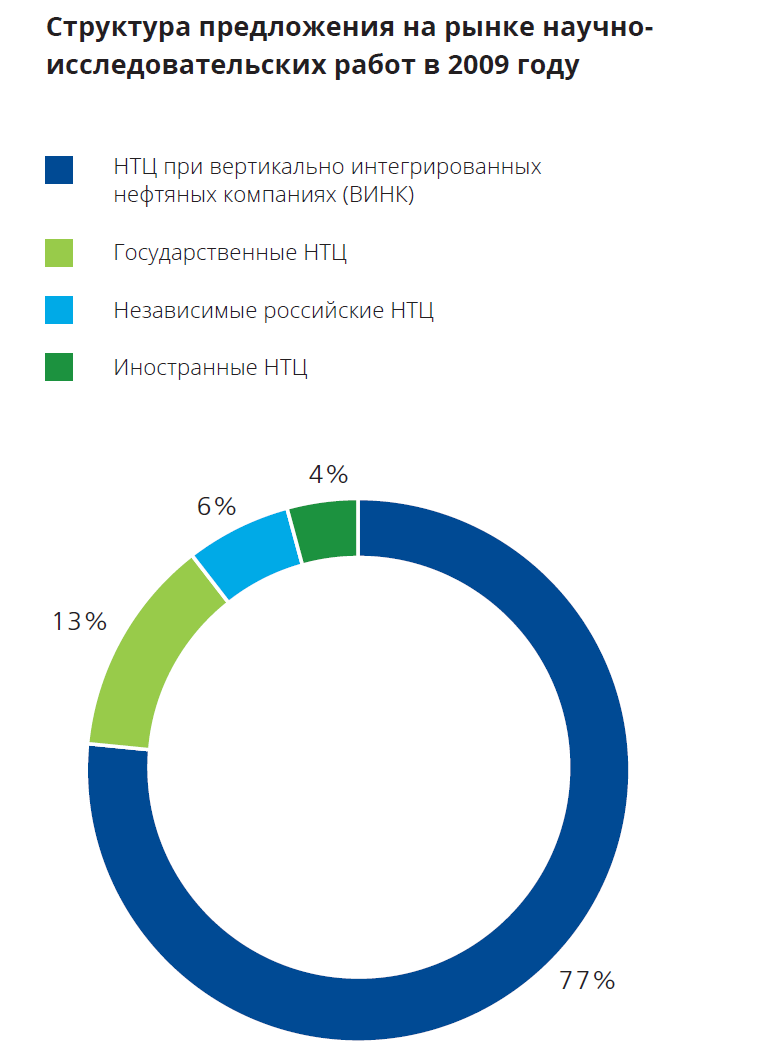
\includegraphics[width=0.8\textwidth]{int0}   
	\label{fig:int0} 
\end{figure}   

Итак, мы видим, что несмотря на определенную фактическую ориентацию отрасли на импортные технологии, доля НТЦ зарубежных нефтесервисных компаний невысока, в то время как как доля НТЦ при крупных российских вертикально интегрированных нефтегазовых компаниях превышают суммарную долю для НТЦ всех остальных типов.
Это не означает, что отрасль использует отечественные технологии, а означает лишь, что крупные игроки отрасли предпочитают осваивать и адаптировать импортные технологии своими собственными силами.
Учитывая текущую структуру рынка разработки технологий в нефтегазовой сфере России, пристальное внимание следует как раз таки уделить деятельности независимых НТЦ, причем с учетом времени их функционирования на рынке.
Так можно выявить скрытые технологические тренды и актуальные производственно-технологические запросы в нефтедобывающей отрасли России.
Разумеется, если НТЦ достаточно молод, например, функционирует на рынке не более 5 лет, то это вовсе не означает, что такая компания не может демонстрировать высокую эффективность, но при этом все же очевидно, что деятельность достаточно молодых компаний на рынке требует дополнительного анализа с точки зрения оценки эффективности и выявления перспективных трендов.

 \begin{figure}[H]
 	\caption{Операционные затраты НТЦ на одного технического специалиста, в млн рублей, 2009}
	\centering     
	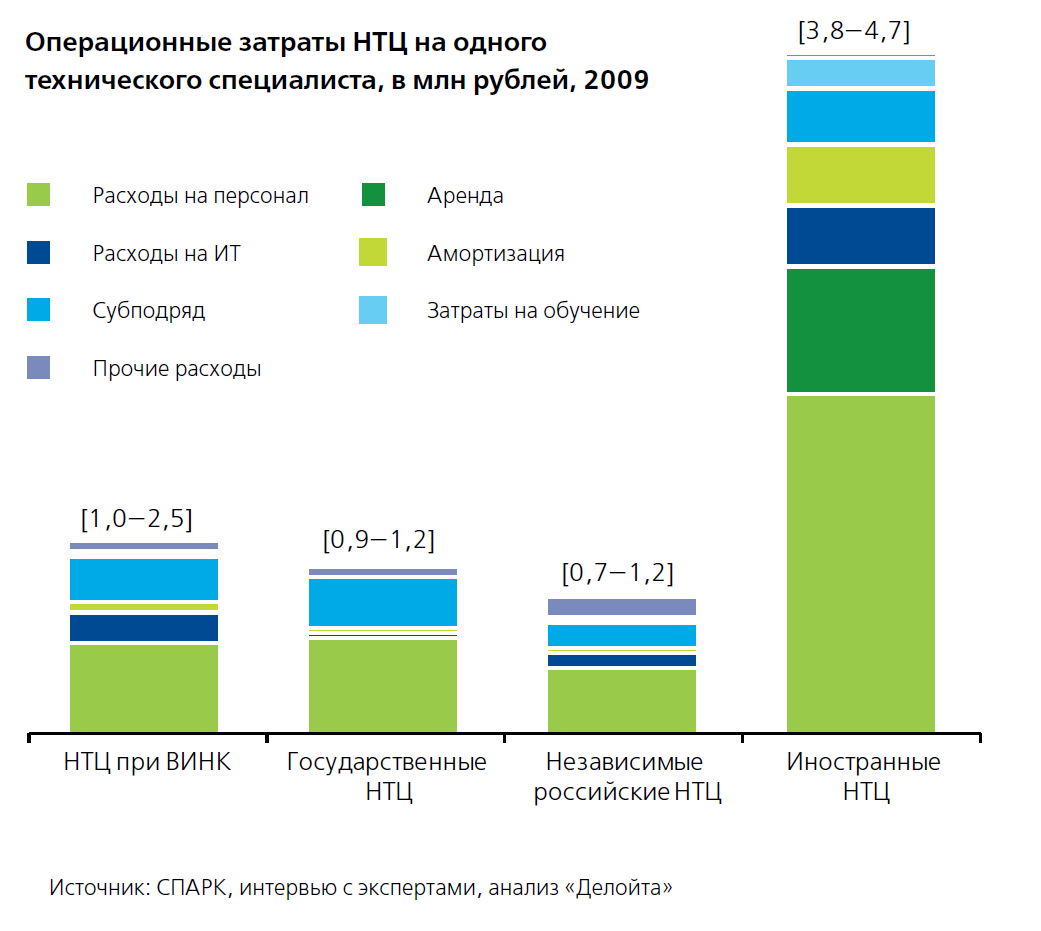
\includegraphics[width=0.8\textwidth]{int2}   
	\label{fig:int2} 
\end{figure}   

Перейдем к описанию критериев эффективности деятельности НТЦ в долгосрочном плане, связанных с собственно производимой НТЦ продукцией в виде новых технологий.
Для этого рассмотрим подход, основанный на анализе цифровых артефактов деятельности НТЦ, в первую очередь различного рода документов в электронном формате, отражающих результаты деятельности НТЦ и доступных для анализа из открытых источников.
К такого рода цифровым артефактам могут быть отнесены:  

\begin{itemize} 
	\tightlist 
	\item документы отраслевых электронных библиотек; 
	\item патенты; 
	\item статьи в отраслевых научных изданиях; 
	\item другие материалы и документы, относящиеся к деятельности нефтегазовой отрасли, имеющиеся в открытом доступе, в первую очередь в сети интернет 
\end{itemize}  

Все указанные документы могут быть подвергнуты компьютерному анализу, в первую очередь высоко-перспективным методом тематического моделирования, суть которого состоит в использовании би-кластеризации, то есть одновременной кластеризации слов и документов по их семантической близости.
При этом как правило используется скрытое размещение Дирихле, которое хотя и удобно для алгоритмических компьютерных вычислений при проведении тематического моделирования, но не вполне обосновано с лингвистической точки зрения.

Результаты тематического моделирования, проведенного автором настоящей работы, для статей во всех выпусках журнала ``Нефтегазовое хозяйство'' за период с 2008 по 2016 годы (что упоминалось уже в настоящей главе ранее) показали, что вопреки изначальному предположению о плавной эволюции выявляемых в рамках тематического моделирования тематик от номера к номеру, в различных номерах журнала были зафиксированы принципиально различные тематики.
Означает ли это, что указанный журнал в каждом новом выпуске концентрируется на новейших технологических достижениях и не производит отсылку к устаревшим и не использующимся технологическим подходам? И да, и нет.
Конъюктурная составляющая при отборе редакцией журнала публикаций с целью повышения привлекательности издания в широких кругах деятелей нефтегазовой и смежных областей очевидна.
В этом в значительной степени и состоит суть любой, в том числе и узкопрофильной, специализированной журналистики.
В то же время о судьбе упомянутых однократно технологий судить по таким однократным публикациям нельзя.
Были ли они отвергнуты в практическом применении или были опробованы и показали свою несостоятельность? 
Или, быть может, прочно вошли за анализируемый период времени длительностью в 8 лет в инструментарий нефтедобывающей отрасли? 
Такие выводы на основе проанализированной информации сделаны быть не могут.
В чем же состоит выход? 
Он состоит в анализе более широкого круга документов, от патентов до тезисов докладов на отраслевых конференциях.
Указанные документы могут быть подвергнуты кластерному анализу с применением различных алгоритмов.
При этом если речь идет об использовании классификации с обучающим шаблоном (``с учителем''), то в качестве обучающего шаблона могут быть выбраны экспертные описания основных современных технологических трендов и инновационных тематик в нефтегазовой отрасли.
Те же совокупности анализируемых документов, которые не войдут в определенные таким образом классы (кластеры), не должны рассматриваться априори как ``шум'', а должны быть подвергнуты дополнительному анализу на предмет того, что они на самом деле представляют собой свидетельства (цифровые артефакты) латентных инновационно-технологических трендов.

На базе такой выполненной кластеризации (классификации) документов (цифровых артефактов инновационно-технологического развития нефтегазовой отрасли) могут быть определены многокритериальные интегральные числовые показатели эффективности деятельности конкретных НТЦ, вычисляемые на основе долей распределения цифровых артефактов, произведенных сотрудниками данного НТЦ, по кластерам (классам).
Изменение таких распределений во времени могут служить основой для апостериорного прогнозного моделирования эффективности деятельности конкретных НТЦ в будущие периоды времени.

Отдельной темой, хотя и относящейся к технической стороне настоящего исследования, является обеспечение информационного обмена, доступа к документам (цифровым артефактам) и их предобработка, включая приведение в единообразные электронные форматы и стемминг.

Все эти вопросы и будут рассмотрены в последующих главах настоящей работы.
